\chapter{参考轨迹保留的预算约束多分支条件引导与安全回退方法}

MatterGen 将晶体生成表示为原子类型、周期坐标与晶胞三个相互耦合字段上的扩散过程，并可通过属性条件实现材料逆向生成\citep{zeni2025}。在条件采样阶段，分类器无关引导（classifier-free guidance，CFG）利用条件得分与无条件得分之差增强条件响应\citep{ho2022}。引导强度过低可能削弱目标属性约束，过高则可能放大模型误差并损害结构质量。因此，如何在属性符合度与生成质量之间配置引导强度，是 MatterGen 推理阶段的重要控制问题。

本章围绕这一问题展开。研究最初从多字段残差驱动的在线自适应 CFG 出发，随后通过反事实 Oracle、风险校准、时间阶段与字段归因实验，逐步识别在线控制不稳定的原因。在这些证据基础上，本文将问题由``在生成过程中提前预测最优引导强度''重新表述为``在有限推理预算内保留基准轨迹、展开少量候选并在终点约束下选择''。最终形成参考轨迹保留的预算约束多分支条件引导与安全回退方法（Reference-Preserved Budget-Constrained Multi-Branch Guidance with Safety-Constrained Fallback），并以固定双候选分支策略（Fixed-K2）作为本章最终方法。

需要预先说明，本章中的目标属性误差由冻结的 CHGNet 磁性密度代理模型计算\citep{deng2023}，能量高于凸包值（energy above hull，E-hull）与稳定性主要由 Matter\allowbreak Sim 代理评价器给出\citep{yang2024mattersim}。这些结果是冻结协议下的代理模型证据，不等同于密度泛函理论（DFT）或实验验证；本章所有实验的 \texttt{DFT\_VERIFIED} 均为 \texttt{false}。

\section{问题定义与研究动机}

\subsection{MatterGen 中的固定条件引导}

设扩散采样第 \(t\) 步的无条件得分为 \(s_{\mathrm{uncond}}(x_t,t)\)，给定目标条件 \(c\) 后的条件得分为 \(s_{\mathrm{cond}}(x_t,t,c)\)。标准 CFG 按下式构造用于反向扩散的得分：

\[
s_{\mathrm{cfg}}(x_t,t,c)
=s_{\mathrm{uncond}}(x_t,t)
+g\left[s_{\mathrm{cond}}(x_t,t,c)-s_{\mathrm{uncond}}(x_t,t)\right],
\]

其中 \(g\) 为 CFG 强度。固定 CFG=2.0 的 MatterGen 参考基线记为 C0，即其在全部采样步骤中固定 \(g_0=2.0\)。MatterGen 的得分不是单一欧氏向量，而由三个主要字段组成：原子类型 \texttt{atomic\_numbers}、周期坐标 \texttt{pos} 和晶胞 \texttt{cell}。因此，可将第 \(f\) 个字段的引导写为

\[
s_{\mathrm{cfg},f}
=s_{\mathrm{uncond},f}+g\left(s_{\mathrm{cond},f}-s_{\mathrm{uncond},f}\right),
\qquad
f\in\{a,p,H\},
\]

其中 \(a,p,H\) 分别表示原子类型、位置与晶胞字段，\(H\) 与第4章采用的晶胞矩阵记号一致。

固定 \(g=2.0\) 的优点是实现简单、计算预算稳定且便于复现，但它对所有样本、所有反向扩散时刻以及三个字段采用同一强度。这隐含了一个较强假设：不同样本和状态对条件信号的需求基本一致。实际采样中，条件得分与无条件得分的差异随字段和时间明显变化，固定引导并未利用这些在线信息。由此形成本文最初的研究问题：是否存在随样本、采样阶段或字段变化的更优条件引导策略？

\subsection{研究假设与评价目标}

本文最初假设，条件得分与无条件得分之间的残差可以反映当前状态下条件信息的作用强弱。若残差相对其历史水平增大，可适当提高引导；若残差减小，则降低引导以避免过度放大。该假设不需要重新训练 MatterGen，也不引入属性梯度或外部物理力，属于推理阶段的闭环采样控制。

本章以目标磁性密度的绝对误差作为属性误差，对样本集合取均值得到 Property MAE：

\[
E_{\mathrm{prop}}=\frac{1}{n}\sum_{i=1}^{n}
\left|\hat c_i-c_i^{\star}\right|,
\]

其中 \(\hat c_i\) 为冻结属性代理模型的预测值，\(c_i^{\star}\) 为目标条件。同时报告 E-hull、Stable、Novel、Unique、NUS（Novel、Unique 且 Stable）与 Validity 等质量指标。方法判断不只关注总体均值，还使用配对差异、20 000 次自助法置信区间、伤害率和尾部退化，以避免少数大幅改善掩盖大量轻微损害。

\section{多字段残差驱动的在线自适应 CFG}

\subsection{字段残差与共享控制量}

对于每个字段 \(j\in\{a,p,H\}\)，V1 首先计算条件与无条件得分差的均方根残差：

\[
\Delta_j(t)=
\sqrt{\operatorname{mean}\left[
\left(s_{\mathrm{cond},j}(t)-s_{\mathrm{uncond},j}(t)\right)^2
\right]}.
\]

三个字段具有不同张量形状，因而先分别降维为标量，再进行等权平均：

\[
\bar\Delta(t)=\frac{1}{3}
\left[\Delta_a(t)+\Delta_p(t)+\Delta_H(t)\right].
\]

需要强调的是，V1 虽然分别计算三个字段的残差，但最终只输出一个全局共享 CFG，而不是三个独立的字段引导系数。也就是说，字段残差用于估计共同的控制信号，得到的 \(g_t\) 仍同时作用于 \texttt{atomic\_numbers}、\texttt{pos} 和 \texttt{cell}。

MatterGen 的预测器与校正器调用具有不同统计尺度。V1 因此为两个阶段分别维护指数移动平均（exponential moving average，EMA）。记阶段 \(q\in\{\mathrm{predictor},\mathrm{corrector}\}\)，则

\[
m_q(t)=
\begin{cases}
\bar\Delta(t), & \text{该阶段首次观测},\\
\beta m_q(t-1)+(1-\beta)\bar\Delta(t), & \text{其他情况}.
\end{cases}
\]

在实现中先用当前残差更新 EMA，再计算相对比值与引导强度：

\[
r_t=\frac{\bar\Delta(t)}{m_q(t)+\varepsilon},
\]

\[
u_t=\operatorname{clip}\left(1+\alpha(r_t-1),0.25,4\right),
\]

\[
g_t=\operatorname{clip}\left(g_0u_t,g_{\min},g_{\max}\right).
\]

冻结的 V1 参数为 \(g_0=2.0\)、\(\alpha=0.5\)、\(\beta=0.95\)、\(\varepsilon=10^{-6}\)，最终范围为 \([0,5]\)。残差非法或统计量非有限时，控制器回到基础引导。每个新样本开始时重新初始化 EMA，不跨样本传递状态。

\subsection{V1 实验结果与稳定性问题}

V1 的历史 Formal256 在 256 对相同随机种子上表现出方向性质量改善：平均 E-hull 从 0.143667 eV/atom 降至 0.140232 eV/atom，Stable 从 41.02\% 增至 46.88\%，NUS 从 22.27\% 增至 25.78\%。然而，三项配对置信区间均跨越零：E-hull 差异的 95\% 置信区间为 \([-0.017926,0.011030]\)，Stable 为 \([-1.56,13.28]\) 个百分点，NUS 为 \([-2.73,9.77]\) 个百分点。因此，该批结果只能说明方向性改善，不能解释为统计上稳健的普遍优势。该历史批次也没有保存可用于独立核验的目标属性预测，不能回填 Property MAE。

随后在预先注册的 8 个新配对种子上进行组件诊断。完整 V1 的 Property MAE 从 C0 的 0.031306 降至 0.019655，但改善区间仍跨越零；与此同时，E-hull 从 0.043371 增至 0.085877 eV/atom，Stable 从 100\% 降至 62.5\%，未复现 Formal256 的质量改善方向。由于样本量较小，该批结果不能单独建立普遍统计结论，但它足以否定``V1 已在跨批次条件下稳定改善质量''的表述。

上述结果暴露了关键问题：在线残差规则能够改变生成结果，且在部分批次呈现有利方向，但收益对样本集合敏感。下一步需要区分两种可能性：一是控制规则没有正确识别有利偏离；二是固定 CFG=2.0 已经接近最优，根本不存在足够的样本级优化空间。为回答这一问题，本文进一步开展反事实 Oracle 实验。

\section{反事实 Oracle 与引导优化空间}

\subsection{实验设计}

反事实 Oracle V3 在 32 条新种子轨迹的 8 个预注册决策时刻上，比较三种冻结候选动作：降低引导 \texttt{DOWN}（CFG=1.75）、保持基准 \texttt{KEEP}（CFG=2.0）和提高引导 \texttt{UP}（CFG=2.25）。每个候选均从相同扩散状态出发，并恢复相同的 CPU/CUDA 随机数状态，从而使差异只来自引导动作。

实验同时构造两类选择器。短视野选择器只观察候选执行 15 个反向步骤后的代理结果，代表可能在线使用的局部反馈；完整终点 Oracle 则将候选保持至采样终点，并在事后选择最终属性误差最低的动作。后者拥有部署时不可获得的未来信息，因而只表示优化空间上界，不能视为可部署算法。

在 256 个短视野状态中，完整展开其中 64 个状态，得到 192 个完整候选终点。所有完整 \texttt{KEEP} 分支与对应固定 CFG=2.0 终点实现了原子类型完全一致、坐标与晶胞最大绝对误差均为 0 的配对核验。

\subsection{结果与机制解释}

完整终点 Oracle 将 CFG=2.0 的 Property MAE 从 0.030446 降至 0.022158，相对改善 27.22\%。其动作分布包含 23.44\% 的 \texttt{DOWN}、62.50\% 的 \texttt{KEEP} 和 14.06\% 的 \texttt{UP}，说明更优动作同时依赖样本与扩散时刻，而不是统一地增大或减小 CFG。这一结果回答了前述存在性问题：固定 CFG=2.0 并非所有状态的终点最优选择，样本级引导优化空间客观存在。

但局部反馈并不能可靠识别这一空间。短视野标签与完整终点标签的一致率为 62.5\%；按照短视野标签执行到终点后，冻结属性目标反而相对 CFG=2.0 恶化 6.90\%，未达到预注册的至少 5\% 改善门槛。短视野选择还产生 15.63\% 的属性伤害率。由此可见，局部候选在短时间内的有利变化并不必然延续到最终晶体，在线控制面临明显的短期代理---长期结果错配。

该实验的结论不是``没有更好的 CFG''，而是``最终更好的 CFG 难以由当前中间状态和短视野结果稳定识别''。完整终点 Oracle 的 27.22\% 改善是机制上界，不能作为部署性能。该转折使研究重点由继续调整残差公式，转向分析错误动作的风险来源及更保守的选择机制。

\section{在线自适应引导不稳定性的机制分析}

图3-1汇总了从 V1 到最终 Fixed-K2 的证据演化。各阶段不是相互独立的新算法，而是围绕残差信号、风险识别、时间阶段和字段解耦四类失败假设展开的连续机制实验。

\begin{figure}
\centering
\pandocbounded{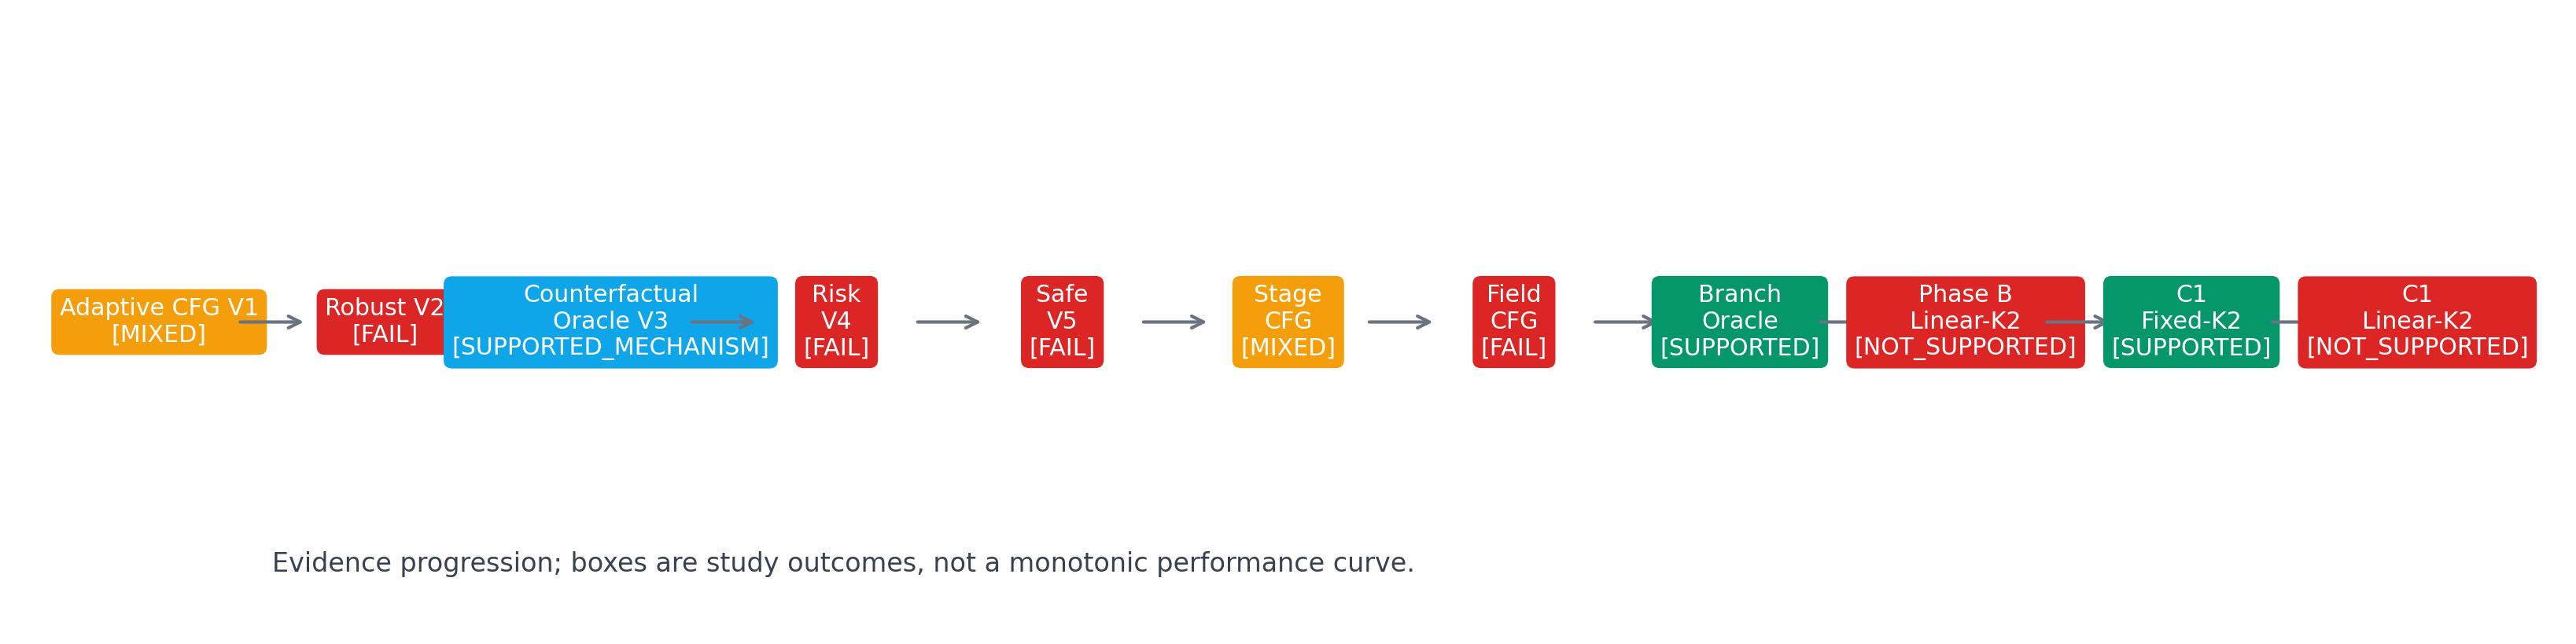
\includegraphics[keepaspectratio,alt={图3-1 创新点1的证据演化：方框表示各阶段冻结结论，而非单调性能曲线}]{../../../thesis_release/innovation1/figures/I1_F6_evidence_progression.png}}
\bicaption{创新点1的证据演化：方框表示各阶段冻结结论，而非单调性能曲线}{Evidence Evolution of Innovation 1: Boxes Denote Frozen Stage Conclusions Rather Than a Monotonic Performance Curve}
\end{figure}


\begin{longtable}[]{@{}
  >{\raggedright\arraybackslash}p{(\linewidth - 10\tabcolsep) * \real{0.1579}}
  >{\raggedright\arraybackslash}p{(\linewidth - 10\tabcolsep) * \real{0.1579}}
  >{\raggedleft\arraybackslash}p{(\linewidth - 10\tabcolsep) * \real{0.2105}}
  >{\raggedright\arraybackslash}p{(\linewidth - 10\tabcolsep) * \real{0.1579}}
  >{\raggedright\arraybackslash}p{(\linewidth - 10\tabcolsep) * \real{0.1579}}
  >{\raggedright\arraybackslash}p{(\linewidth - 10\tabcolsep) * \real{0.1579}}@{}}
 \bicaption{在线自适应 CFG 探索与机制实验汇总}{Summary of Online Adaptive CFG Exploration and Mechanistic Experiments}\label{tab:3-1}\\

        \toprule
        \noalign{}
\begin{minipage}[b]{\linewidth}\raggedright
实验
\end{minipage} & \begin{minipage}[b]{\linewidth}\raggedright
核心问题
\end{minipage} & \begin{minipage}[b]{\linewidth}\raggedleft
数据规模
\end{minipage} & \begin{minipage}[b]{\linewidth}\raggedright
主要发现
\end{minipage} & \begin{minipage}[b]{\linewidth}\raggedright
冻结状态
\end{minipage} & \begin{minipage}[b]{\linewidth}\raggedright
对下一阶段的作用
\end{minipage} \\
\midrule\noalign{}
\endfirsthead
        \toprule
        \noalign{}
\begin{minipage}[b]{\linewidth}\raggedright
实验
\end{minipage} & \begin{minipage}[b]{\linewidth}\raggedright
核心问题
\end{minipage} & \begin{minipage}[b]{\linewidth}\raggedleft
数据规模
\end{minipage} & \begin{minipage}[b]{\linewidth}\raggedright
主要发现
\end{minipage} & \begin{minipage}[b]{\linewidth}\raggedright
冻结状态
\end{minipage} & \begin{minipage}[b]{\linewidth}\raggedright
对下一阶段的作用
\end{minipage} \\
\midrule\noalign{}
\endhead


\bottomrule\noalign{}
\endlastfoot
Adaptive CFG V1 & 多字段残差能否直接控制共享 CFG & Formal256 + fresh8 & 历史方向性改善未在新批次稳定复现 & MIXED & 暴露跨批次稳定性问题 \\
Robust V2 & 归一化、置信回退和限速能否降低伤害 & P0=32 & 未降低旧 V1 的三类伤害率，属性护栏失败 & FAIL & 表明原始残差幅值不足以作为稳定控制信号 \\
Counter\allowbreak factual Oracle V3 & 更优的样本/时刻引导是否存在 & 32 seeds，64 个完整状态 & 完整 Oracle 有 27.22\% 优化空间，但短视野选择失效 & SUP\allowbreak PORTED\_MECHAN\allowbreak ISM & 将问题转化为``如何识别有利偏离'' \\
Risk-Calibrated V4 & 风险模型能否过滤有害动作 & 96 trajectories & 无操作点同时达到覆盖率与伤害率门槛 & FAIL & 转向更保守的安全选择 \\
Safe Selection V5 & 显式安全校准能否保留收益 & 128 trajectories & 验证集无操作点通过冻结门槛 & FAIL & 转向时间与字段归因 \\
Stage-Calibrated CFG & 有利偏离是否集中在特定阶段 & calibration32 + P0=32 & 脉冲改善属性但破坏质量，阶段特异性不成立 & MIXED & 支持使用有限脉冲作为候选，而非单轨控制 \\
Field-Decoupled CFG & 不同字段能否独立控制 & calibration=48 & 属性与伤害均为多字段效应，无策略通过门槛 & FAIL & 为分支候选库提供字段归因 \\
\end{longtable}
\subsection{残差信号稳健性}

Robust Adaptive CFG V2 针对 V1 的跨字段尺度和快速波动问题进行了预注册改造。首先使用 64 个历史 C0 样本进行确定性重放，将三个字段残差按预测器/校正器、字段以及 20 个时间区间分别转换为对数标准分数；随后以三个字段标准分数的中位数作为聚合量，并为预测器和校正器分别维护 \(\beta=0.95\) 的 EMA。控制器根据残差偏离基准死区的程度与字段一致性计算置信度，置信度为零或残差非法时精确回到 CFG=2.0。最终引导范围冻结为 \([1.5,2.5]\)，相邻得分调用的变化幅度不超过 0.05，且关闭阶段门控。

在 32 个全新 P0 配对样本上，V2 的稳健版本 \texttt{A\_ROBUST} 相对 C0 的 E-hull、Stable 和属性伤害率分别为 43.75\%、18.75\% 和 53.13\%，与旧 V1 在该批次上的对应伤害率完全相同，未满足``至少一类伤害率相对下降 30\%''的预注册门槛。其 Property MAE 为 0.029870，高于 C0 的 0.023210，也违反了属性误差最多恶化 10\% 的护栏。该结果表明，时间归一化、中位数聚合、置信回退和限速改善了控制形式，但没有解决跨样本的错误动作识别问题；原始残差的幅值及其平滑变换仍不足以构成稳定的在线控制信号。

\subsection{风险校准与安全选择}

Oracle 已证明有利偏离存在，因此 V4 不再直接预测最优动作，而是估计动作的收益与伤害风险，并仅在低风险区域内允许偏离。其冻结门槛要求所选操作点覆盖率不低于 15\%，且被选动作的属性伤害率不高于 10\%。在 96 条完整轨迹上，没有验证操作点同时满足二者，故实验在离线阶段停止，未进入新 P0 或 Formal256。

V5 进一步采用保守的候选安全选择，将收益预测与经过校准的伤害概率联合约束。数据集包含 128 条轨迹，但预注册候选网格中仍没有验证操作点同时满足覆盖率与伤害率门槛，因此测试集、P0 和 Formal256 均未运行。V4 与 V5 共同说明：误报一个``有利偏离''的代价较高，而当前手工设计的分支前特征、样本规模和安全校准方法不能稳定筛出这类偏离。该结论只约束本研究中的特征与协议，不能外推为所有自适应控制器均不可能成功。

\subsection{时间阶段与字段维度分析}

Stage-Calibrated CFG 研究较低引导是否只在特定扩散阶段有效。冻结候选包括全程 CFG=1.9、从第 400 步起永久降至 1.9，以及从第 400 步起持续 100 步的有界脉冲。Fresh P0 的结果见表3-2。


\begin{longtable}[]{@{}
  >{\raggedright\arraybackslash}p{(\linewidth - 10\tabcolsep) * \real{0.1304}}
  >{\raggedleft\arraybackslash}p{(\linewidth - 10\tabcolsep) * \real{0.1739}}
  >{\raggedleft\arraybackslash}p{(\linewidth - 10\tabcolsep) * \real{0.1739}}
  >{\raggedleft\arraybackslash}p{(\linewidth - 10\tabcolsep) * \real{0.1739}}
  >{\raggedleft\arraybackslash}p{(\linewidth - 10\tabcolsep) * \real{0.1739}}
  >{\raggedleft\arraybackslash}p{(\linewidth - 10\tabcolsep) * \real{0.1739}}@{}}\bicaption{Stage-Calibrated CFG 的 Fresh P0 结果}{Fresh P0 Results of Stage-Calibrated CFG}\label{tab:3-2}\\

        \toprule
        \noalign{}
\begin{minipage}[b]{\linewidth}\raggedright
策略
\end{minipage} & \begin{minipage}[b]{\linewidth}\raggedleft
Property MAE ↓
\end{minipage} & \begin{minipage}[b]{\linewidth}\raggedleft
E-hull (eV/atom) ↓
\end{minipage} & \begin{minipage}[b]{\linewidth}\raggedleft
Stable ↑
\end{minipage} & \begin{minipage}[b]{\linewidth}\raggedleft
NUS ↑
\end{minipage} & \begin{minipage}[b]{\linewidth}\raggedleft
Validity ↑
\end{minipage} \\
\midrule\noalign{}
\endfirsthead
        \toprule
        \noalign{}
\begin{minipage}[b]{\linewidth}\raggedright
策略
\end{minipage} & \begin{minipage}[b]{\linewidth}\raggedleft
Property MAE ↓
\end{minipage} & \begin{minipage}[b]{\linewidth}\raggedleft
E-hull (eV/atom) ↓
\end{minipage} & \begin{minipage}[b]{\linewidth}\raggedleft
Stable ↑
\end{minipage} & \begin{minipage}[b]{\linewidth}\raggedleft
NUS ↑
\end{minipage} & \begin{minipage}[b]{\linewidth}\raggedleft
Validity ↑
\end{minipage} \\
\midrule\noalign{}
\endhead


\bottomrule\noalign{}
\endlastfoot
C0，恒定 2.0 & 0.043425 & 0.064246 & 75.00\% & 43.75\% & 100\% \\
全程 1.9 & 0.035938 & 0.095755 & 56.25\% & 28.13\% & 100\% \\
第400步后永久 1.9 & 0.035973 & 0.170068 & 59.38\% & 46.88\% & 100\% \\
第400--499步脉冲 1.9 & 0.036328 & 0.122792 & 43.75\% & 28.13\% & 100\% \\
\end{longtable}
三种低引导策略均降低了平均属性误差，但均引入至少一项明显质量退化。脉冲相对 C0 的平均属性增益为 0.007097，而 95\% 自助法区间 \([-0.003456,0.017458]\) 跨越零；其 E-hull 几乎翻倍，Stable 降低 31.25 个百分点，NUS 降低 15.63 个百分点。脉冲与全程 1.9 的 Property MAE 基本相当，脉冲相对恒定策略的平均属性增益为 \(-0.000391\)，区间同样跨越零。因此，实验支持``较低 CFG 会改变属性---质量权衡''，但不支持该收益具有明确的阶段特异性。

Field-Decoupled CFG 则将三个字段的引导分别记为 \(g_a,g_p,g_H\)。首先进行实现等价性检查：令 \(g_a=g_p=g_H=2.0\) 时，输出原子类型完全一致，位置与晶胞的最大绝对误差均为 0，从而排除字段化实现自身引入的差异。随后在 48 个校准样本上评价单字段、双字段、全局恒定和脉冲候选。

字段归因结果显示，属性收益的正向贡献约 40.24\% 来自原子类型字段、59.76\% 来自位置字段，晶胞字段未产生正向贡献；质量伤害的聚合归因约 54.72\% 来自位置、42.37\% 来自晶胞、2.91\% 来自原子类型。也就是说，属性改善不是单一原子字段效应，质量损害也不是单一晶胞字段效应。最终 12 个候选中没有策略同时通过属性保持、收益保留、物理质量和基准护栏，因而 P0 与 Formal256 均按协议停止。该结果说明，简单字段解耦不足以得到稳定增益，但它为后续候选分支的设计提供了可解释的字段级干预方式。

\section{参考轨迹保留的预算约束多分支条件引导与安全回退}

\subsection{问题重述与总体思路}

前述实验表明，在线自适应引导的主要困难不是缺少可利用的优化空间，而是在终点结果未知时提前决定何时、以何种方式偏离 C0。错误偏离可能改变后续全部随机演化，仅在后续步骤将 CFG 恢复为 2.0 并不能恢复原始 C0 轨迹。基于这一认识，本文不再要求控制器在单条轨迹上一次性作出不可逆决策，而是保留完整参考轨迹，在固定预算内展开少量可比较候选，并将选择时机延迟到终点。本文将该方法称为``参考轨迹保留的预算约束多分支条件引导与安全回退方法''（Reference-Preserved Budget-Constrained Multi-Branch Guidance with Safety-Constrained Fallback），不另行创造缩写。

最终方法包含四个组成部分：精确保留 C0、共享分支前缀、固定候选预算以及带质量约束的参考回退。其逻辑流程为：

\begin{Shaded}
\begin{Highlighting}[]
\NormalTok{固定 CFG=2.0 运行共享前缀}
\NormalTok{            ↓}
\NormalTok{第 400 步保存完整采样状态与 RNG 状态}
\NormalTok{            ↓}
\NormalTok{  ┌──────── C0 精确参考后缀}
\NormalTok{  ├──────── 候选分支 1}
\NormalTok{  └──────── 候选分支 2}
\NormalTok{            ↓}
\NormalTok{属性代理评价 + 终点质量约束}
\NormalTok{            ↓}
\NormalTok{候选安全且属性改善 → 接受最优候选}
\NormalTok{否则                   → 返回精确 C0}
\end{Highlighting}
\end{Shaded}

这种设计将不确定的在线控制转化为保守的推理时选择：算法不必准确预测唯一最优动作，只需在有限候选中找到一个通过预定义终点约束且优于 C0 的结果；若没有这样的结果，原始基准仍可直接返回。

\subsection{精确参考保留与共享前缀}

设完整采样共 \(T=1000\) 步，分支点为 \(t_b=400\)。将第 \(t_b\) 步的采样状态记为 \(z_{t_b}\)，随机数生成器状态记为 \(\xi_{t_b}\)。方法在分支点保存二者，并对每条后缀分支执行状态克隆与 RNG 恢复：

\[
y_k=F_{P_k}\left(z_{t_b},\xi_{t_b};t_b,T\right),
\qquad k\in\{0,1,\ldots,K\},
\]

其中 \(P_0\) 是始终保持 CFG=2.0 的 C0 后缀，\(P_k\) 是第 \(k\) 个候选策略。所有分支在 \(t_b\) 之前具有完全相同的张量与随机历史，在 \(t_b\) 之后也从同一 RNG 快照开始。C1 实验还额外运行独立的全程 C0，并逐样本检查其与共享前缀 C0 的原子类型、位置和晶胞；128 个确认样本全部通过精确复现检查。

共享前缀避免从初始噪声重复运行 \(K+1\) 条完整轨迹。C0 每个样本需要 2 000 次 MatterGen 得分调用；Fixed-K2 需要前 400 步的 800 次共享调用，以及 C0 和两个候选在后 600 步的 \(3\times1\,200\) 次调用，共 4 400 次，即 C0 的 2.2 倍。该计算量是最终部署成本；Phase B 为收集全部候选监督数据产生的 3.4 倍成本不属于 Fixed-K2 部署成本。

\subsection{冻结候选库与固定双分支}

只有在第 400 步之前与 C0 完全一致的策略才能合法复用共享前缀。最终候选库由表3-3中的四种 100 步脉冲组成。所有脉冲均在第 400--499 步将对应字段从 2.0 降至 1.9，第 500 步起恢复至 2.0。


            \begin{longtable}[]{@{}lrrrll@{}}\bicaption{分支兼容候选策略}{Branch-Compatible Candidate Strategies}\label{tab:3-3}\\

        \toprule
        \noalign{}
策略 & \(g_a\) & \(g_p\) & \(g_H\) & 作用区间 & 含义 \\
\midrule\noalign{}
\endfirsthead
        \toprule
        \noalign{}
策略 & \(g_a\) & \(g_p\) & \(g_H\) & 作用区间 & 含义 \\
\midrule\noalign{}
\endhead


\bottomrule\noalign{}
\endlastfoot
GPulse & 1.9 & 1.9 & 1.9 & 400--499 & 三字段全局脉冲 \\
APulse & 1.9 & 2.0 & 2.0 & 400--499 & 仅原子类型字段脉冲 \\
PPulse & 2.0 & 1.9 & 2.0 & 400--499 & 仅位置字段脉冲 \\
CPulse & 2.0 & 2.0 & 1.9 & 400--499 & 仅晶胞字段脉冲 \\
\end{longtable}
最终 Fixed-K2 冻结选择 \texttt{GPulse+PPulse}，即每个样本只生成两个候选，而不是进行无上限的多样本筛选。固定 \(K=2\) 同时限制推理成本和选择自由度，使方法的收益可以在明确的 2.2 倍预算下评价。

\subsection{终点约束选择与参考回退}

记 \(e(y)=|\hat c(y)-c^{\star}|\) 为候选的属性绝对误差，\(v(y)\) 为有效性，\(s(y)\) 为稳定性二值指标，\(h(y)\) 为 E-hull。对分配给当前方法的候选集合 \(\mathcal P_K\)，冻结的逐样本可接受集合为

\[
\mathcal A=
\left\{y_k\middle|
\begin{aligned}
e(y_0)-e(y_k)&>10^{-6},&
v(y_k)&\ge v(y_0),\\
s(y_k)&\ge s(y_0),&
h(y_k)&\le h(y_0)+0.01
\end{aligned}
\right\},
\]

其中 \(y_0\) 为精确 C0，且候选与 C0 的 E-hull 均须为有限值。最终输出为

\[
y^{\star}=
\begin{cases}
\displaystyle\arg\min_{y_k\in\mathcal A}e(y_k), & \mathcal A\ne\varnothing,\\
y_0, & \mathcal A=\varnothing.
\end{cases}
\]

该逐样本规则直接约束属性改进、有效性、稳定性和 E-hull。NUS 等集合级指标用于确认阶段的整体质量护栏，但不应被误写为逐样本终点选择条件。参考回退的含义也不是``保证物理安全''，而是在当前代理评价和预定义接受条件下，不接受违反约束的候选。

\subsection{算法描述}

\textbf{算法3-1 参考轨迹保留的预算约束多分支条件引导与安全回退}

\begin{Shaded}
\begin{Highlighting}[]
\NormalTok{输入：条件 c；基准引导 g0=2.0；分支点 tb；}
\NormalTok{      候选策略集合 P；分支预算 K；终点接受约束 Q}
\NormalTok{输出：晶体 x*}

\NormalTok{1:  初始化 MatterGen 采样状态 z0 与随机数生成器}
\NormalTok{2:  使用 g0 将基准轨迹推进至 tb}
\NormalTok{3:  保存完整状态 ztb 和 RNG 状态 ξtb}
\NormalTok{4:  恢复 (ztb, ξtb)，使用 g0 完成后缀，得到精确参考 x0}
\NormalTok{5:  对预先分配的 K 个候选策略 Pk：}
\NormalTok{6:      恢复同一 (ztb, ξtb) 并克隆采样状态}
\NormalTok{7:      在冻结区间应用 Pk，其余步骤使用 g0}
\NormalTok{8:      完成采样，得到候选 xk}
\NormalTok{9:  使用冻结属性与质量评价器计算 x0 及全部 xk 的终点指标}
\NormalTok{10: 构造同时满足属性严格改善与质量约束 Q 的候选集合 A}
\NormalTok{11: 若 A 非空，返回其中属性误差最小者}
\NormalTok{12: 否则返回精确参考 x0}
\end{Highlighting}
\end{Shaded}

算法的实现关键是第 3、4、6 步：完整采样状态与 RNG 状态必须同时保存和恢复。若只恢复 CFG 数值而不恢复状态，候选所经历的中间更新已不可逆，不能被称为 C0 回退。

\section{分支兼容 Oracle 与候选预算分析}

\subsection{分支兼容性约束}

早期实验包含多种全程或更早阶段生效的策略，但它们无法从第 400 步的 C0 状态合法分叉。分支兼容性审计因此只保留 GPulse、APulse、PPulse 和 CPulse。审计检查表明，这些候选具有相同的分支点和共同前缀摘要；实现代码在第 400 步保存 RNG、克隆完整状态，并在每个分支执行前恢复 RNG。该约束保证候选比较来自同一起点，也使共享前缀的 2.2 倍计算估计成立。

\subsection{Oracle 上界与 K=2 动机}

在历史数据的独立测试划分 \(n=12\) 上，C0 的 Property MAE 为 0.02879873，使用 SAFE-A 终点规则的分支兼容 Oracle-All 为 0.02004107，相对改善 30.41\%。Oracle-K2 恢复了 100\% 的 Oracle-All 优化空间，而训练划分选出的固定 \texttt{CPulse+GPulse} 在测试集恢复 72.56\%。结果见表3-4。


            \begin{longtable}[]{@{}
  >{\raggedright\arraybackslash}p{(\linewidth - 8\tabcolsep) * \real{0.1579}}
  >{\raggedleft\arraybackslash}p{(\linewidth - 8\tabcolsep) * \real{0.2105}}
  >{\raggedleft\arraybackslash}p{(\linewidth - 8\tabcolsep) * \real{0.2105}}
  >{\raggedleft\arraybackslash}p{(\linewidth - 8\tabcolsep) * \real{0.2105}}
  >{\raggedleft\arraybackslash}p{(\linewidth - 8\tabcolsep) * \real{0.2105}}@{}}\bicaption{分支兼容 Oracle 的测试集结果}{Test-Set Results of the Branch-Compatible Oracle}\label{tab:3-4}\\

        \toprule
        \noalign{}
\begin{minipage}[b]{\linewidth}\raggedright
方法
\end{minipage} & \begin{minipage}[b]{\linewidth}\raggedleft
Property MAE ↓
\end{minipage} & \begin{minipage}[b]{\linewidth}\raggedleft
相对 C0 改善
\end{minipage} & \begin{minipage}[b]{\linewidth}\raggedleft
恢复 Oracle 优化空间
\end{minipage} & \begin{minipage}[b]{\linewidth}\raggedleft
估计计算量
\end{minipage} \\
\midrule\noalign{}
\endfirsthead
        \toprule
        \noalign{}
\begin{minipage}[b]{\linewidth}\raggedright
方法
\end{minipage} & \begin{minipage}[b]{\linewidth}\raggedleft
Property MAE ↓
\end{minipage} & \begin{minipage}[b]{\linewidth}\raggedleft
相对 C0 改善
\end{minipage} & \begin{minipage}[b]{\linewidth}\raggedleft
恢复 Oracle 优化空间
\end{minipage} & \begin{minipage}[b]{\linewidth}\raggedleft
估计计算量
\end{minipage} \\
\midrule\noalign{}
\endhead


\bottomrule\noalign{}
\endlastfoot
C0 & 0.028799 & --- & 0\% & 1.0× \\
Oracle-All & 0.020041 & 30.41\% & 100\% & 3.4× \\
Oracle-K2 & 0.020041 & 30.41\% & 100\% & 2.2× \\
Fixed-K2（Phase A） & 0.022445 & 22.06\% & 72.56\% & 2.2× \\
\end{longtable}
Oracle-K2 在定义上可事后知道每个样本的最佳策略身份，因此它仍是存在性上界，而非可部署的候选分配器。其作用是说明大部分可用优化空间可由很小的候选集合覆盖，从而为 \(K=2\) 提供预算依据。

还需区分两个阶段的固定双候选分支策略：Phase A 使用历史训练划分选出 \texttt{CPulse+GPulse}，最终 C1 的 \texttt{GPulse+PPulse} 则来自后续 Phase B 的独立候选分配流程。二者使用不同样本集合和选择程序，不能相互替换。本章最终方法以 C1 冻结清单中的 \texttt{GPulse+PPulse} 为准。

\section{Fixed-K2 的独立确认结果}

\subsection{确认实验设置}

C1 在所有结果产生前一次性注册了 256 个与历史样本零重叠的随机种子，其中前 128 个构成 C1，后 128 个仅在预注册继续门槛通过时用于 C2。每个 C1 样本均生成精确 C0，并以相同 2.2 倍部署预算比较 Fixed-K2、Random-\allowbreak K2 与 Linear-K2。所有 128 个样本的独立全程 C0 与共享前缀 C0 均通过精确复现检查。

终点属性由冻结 CHGNet 代理模型评价，候选接受使用 3.5.4 节的逐样本规则；集合级 E-hull、Stable、NUS 与 Validity 用于确认质量护栏。Fixed-K2 的主要检验使用 20 000 次确定性配对自助法，差异定义为 C0 属性误差减去 Fixed-K2 属性误差，正值表示 Fixed-K2 更优。

\subsection{属性误差与配对统计}

四种方法的 C1 结果见表3-5和图3-2。Fixed-K2 将 Property MAE 从 0.034796 降至 0.026332，绝对改善 0.008464，相对改善 24.32\%。20 000 次配对自助法得到绝对改善的 95\% 置信区间为 \([0.005817,0.011391]\)，全区间高于零。在 128 个样本中，53 个样本接受了属性更优且通过约束的候选，75 个样本持平或回退 C0，没有样本输出比 C0 更高的属性误差。


            \begin{longtable}[]{@{}
  >{\raggedright\arraybackslash}p{(\linewidth - 14\tabcolsep) * \real{0.0968}}
  >{\raggedleft\arraybackslash}p{(\linewidth - 14\tabcolsep) * \real{0.1290}}
  >{\raggedleft\arraybackslash}p{(\linewidth - 14\tabcolsep) * \real{0.1290}}
  >{\raggedleft\arraybackslash}p{(\linewidth - 14\tabcolsep) * \real{0.1290}}
  >{\raggedleft\arraybackslash}p{(\linewidth - 14\tabcolsep) * \real{0.1290}}
  >{\raggedleft\arraybackslash}p{(\linewidth - 14\tabcolsep) * \real{0.1290}}
  >{\raggedleft\arraybackslash}p{(\linewidth - 14\tabcolsep) * \real{0.1290}}
  >{\raggedleft\arraybackslash}p{(\linewidth - 14\tabcolsep) * \real{0.1290}}@{}}
 \bicaption{C1-128 最终确认结果}{Final Confirmation Results for C1-128}\label{tab:3-5}\\

        \toprule
        \noalign{}
\begin{minipage}[b]{\linewidth}\raggedright
方法
\end{minipage} & \begin{minipage}[b]{\linewidth}\raggedleft
Property MAE ↓
\end{minipage} & \begin{minipage}[b]{\linewidth}\raggedleft
E-hull (eV/atom) ↓
\end{minipage} & \begin{minipage}[b]{\linewidth}\raggedleft
Stable ↑
\end{minipage} & \begin{minipage}[b]{\linewidth}\raggedleft
NUS ↑
\end{minipage} & \begin{minipage}[b]{\linewidth}\raggedleft
Validity ↑
\end{minipage} & \begin{minipage}[b]{\linewidth}\raggedleft
计算量/C0
\end{minipage} & \begin{minipage}[b]{\linewidth}\raggedleft
回退率
\end{minipage} \\
\midrule\noalign{}
\endfirsthead
        \toprule
        \noalign{}
\begin{minipage}[b]{\linewidth}\raggedright
方法
\end{minipage} & \begin{minipage}[b]{\linewidth}\raggedleft
Property MAE ↓
\end{minipage} & \begin{minipage}[b]{\linewidth}\raggedleft
E-hull (eV/atom) ↓
\end{minipage} & \begin{minipage}[b]{\linewidth}\raggedleft
Stable ↑
\end{minipage} & \begin{minipage}[b]{\linewidth}\raggedleft
NUS ↑
\end{minipage} & \begin{minipage}[b]{\linewidth}\raggedleft
Validity ↑
\end{minipage} & \begin{minipage}[b]{\linewidth}\raggedleft
计算量/C0
\end{minipage} & \begin{minipage}[b]{\linewidth}\raggedleft
回退率
\end{minipage} \\
\midrule\noalign{}
\endhead


\bottomrule\noalign{}
\endlastfoot
C0 & 0.034796 & 0.104296 & 58.59\% & 32.81\% & 100\% & 1.0× & 100\% \\
Fixed-K2 & \textbf{0.026332} & \textbf{0.081135} & \textbf{70.31\%} & 37.50\% & 100\% & 2.2× & 58.59\% \\
Linear-K2 & 0.027522 & 0.090528 & 67.97\% & \textbf{39.06\%} & 100\% & 2.2× & 59.38\% \\
Random-\allowbreak K2 & 0.028533 & 0.089172 & 64.84\% & \textbf{39.06\%} & 100\% & 2.2× & 66.41\% \\
\end{longtable}
\begin{figure}
\centering
\pandocbounded{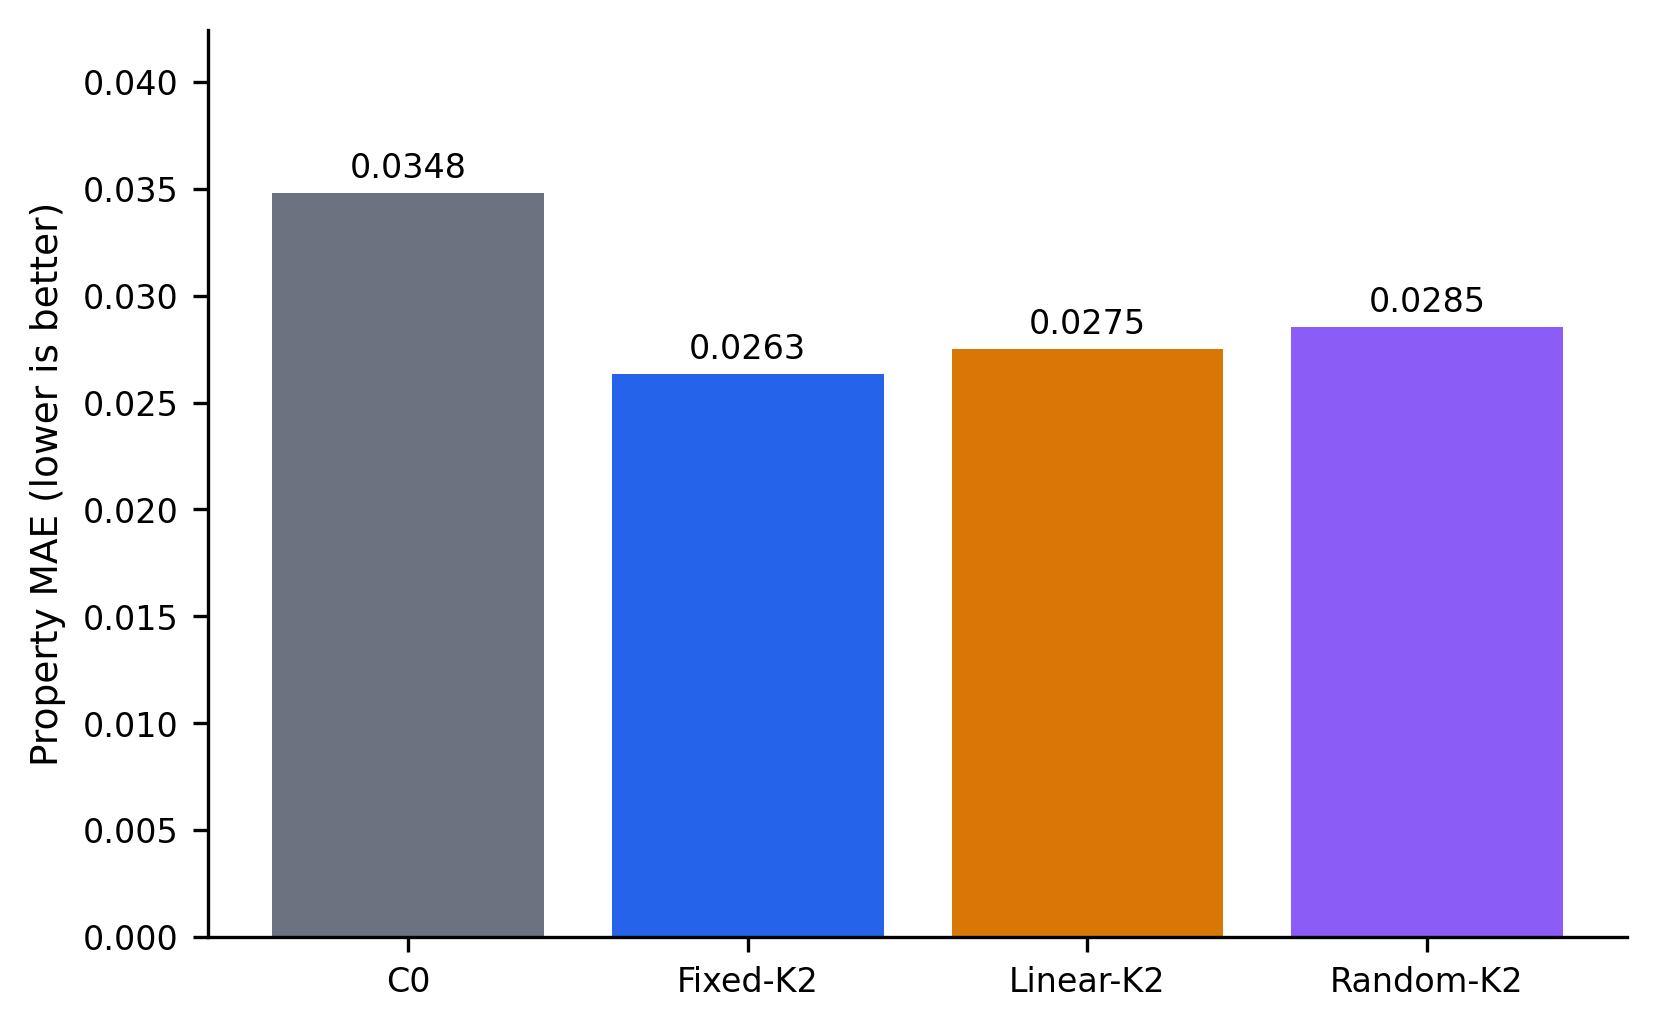
\includegraphics[keepaspectratio,alt={图3-2 C1-128 中 C0、Fixed-K2、Linear-K2 与 Random-\allowbreak K2 的 Property MAE}]{../../../thesis_release/innovation1/figures/I1_F1_c1_property_mae.png}}
\bicaption{C1-128 中 C0、Fixed-K2、Linear-K2 与 Random-\allowbreak K2 的 Property MAE}{Property MAE of C0, Fixed-K2, Linear-K2, and Random-\allowbreak K2 on C1-128}
\end{figure}

图3-3展示 Fixed-K2 与 C0 的逐样本属性误差，图3-4给出配对增益的自助法分布。二者共同说明总体改善不是由少数单边离群值独立驱动，但结论仍应限定在该冻结确认样本与代理评价协议内。

\begin{figure}
\centering
\pandocbounded{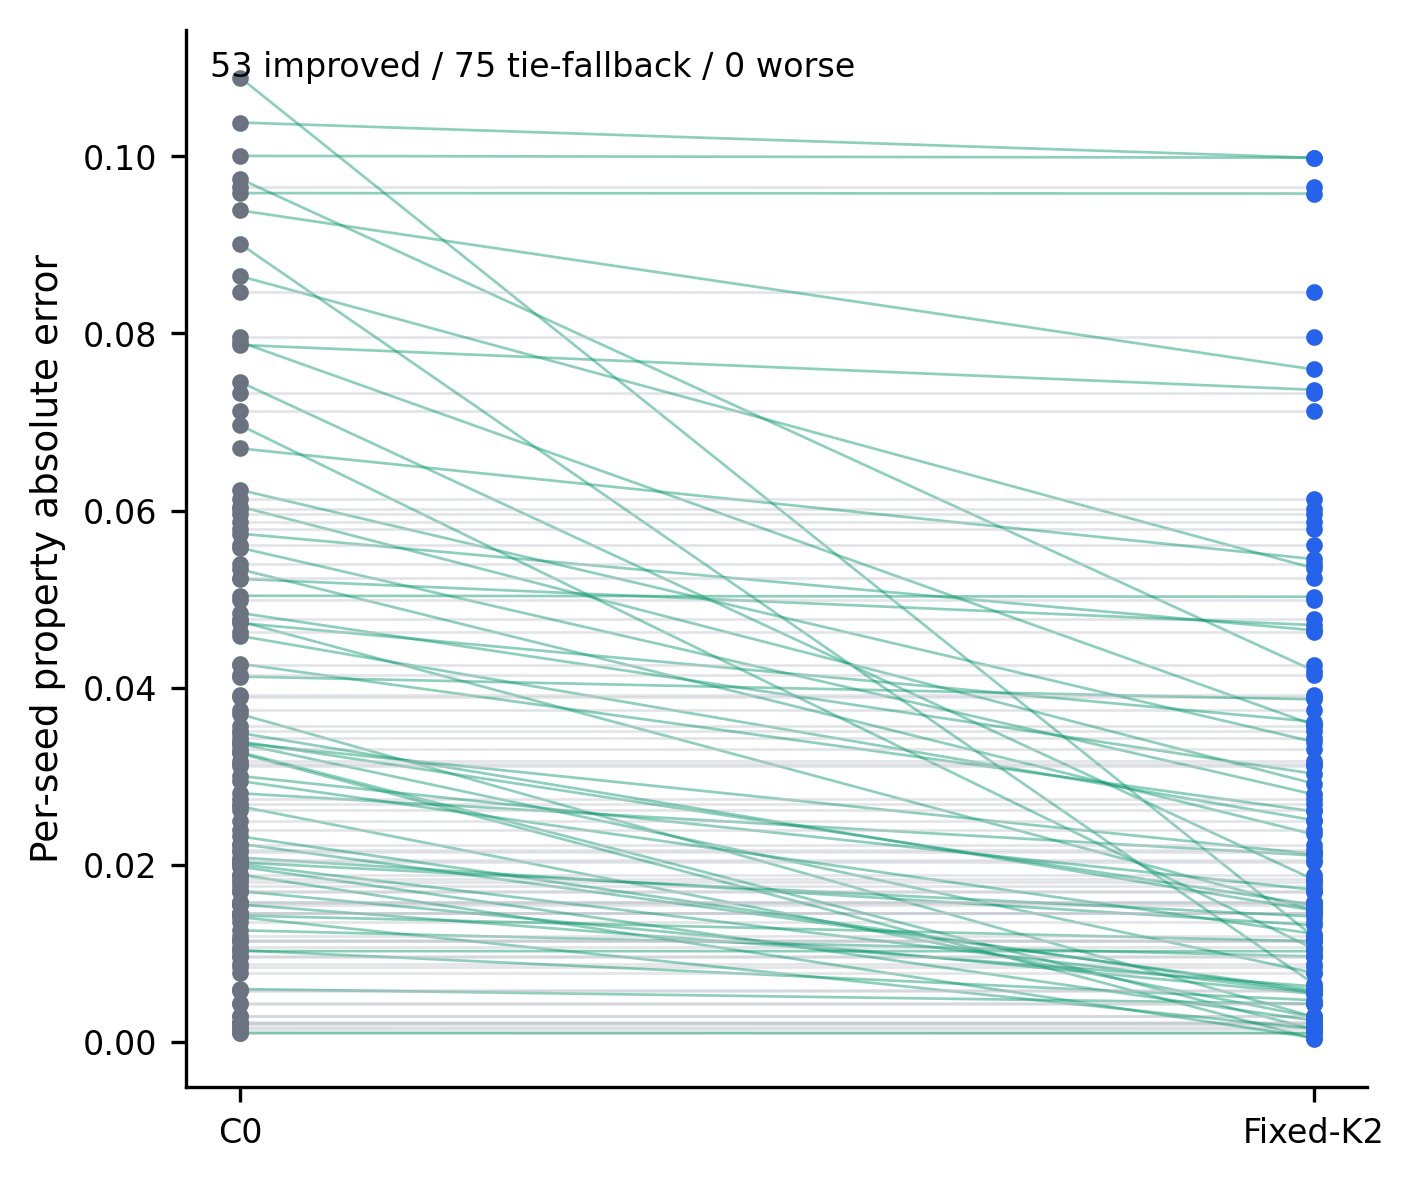
\includegraphics[keepaspectratio,alt={图3-3 Fixed-K2 与 C0 的逐样本属性误差}]{../../../thesis_release/innovation1/figures/I1_F2_fixed_vs_c0_paired.png}}
\bicaption{Fixed-K2 与 C0 的逐样本属性误差}{Per-Sample Property Error of Fixed-K2 and C0}
\end{figure}

\begin{figure}
\centering
\pandocbounded{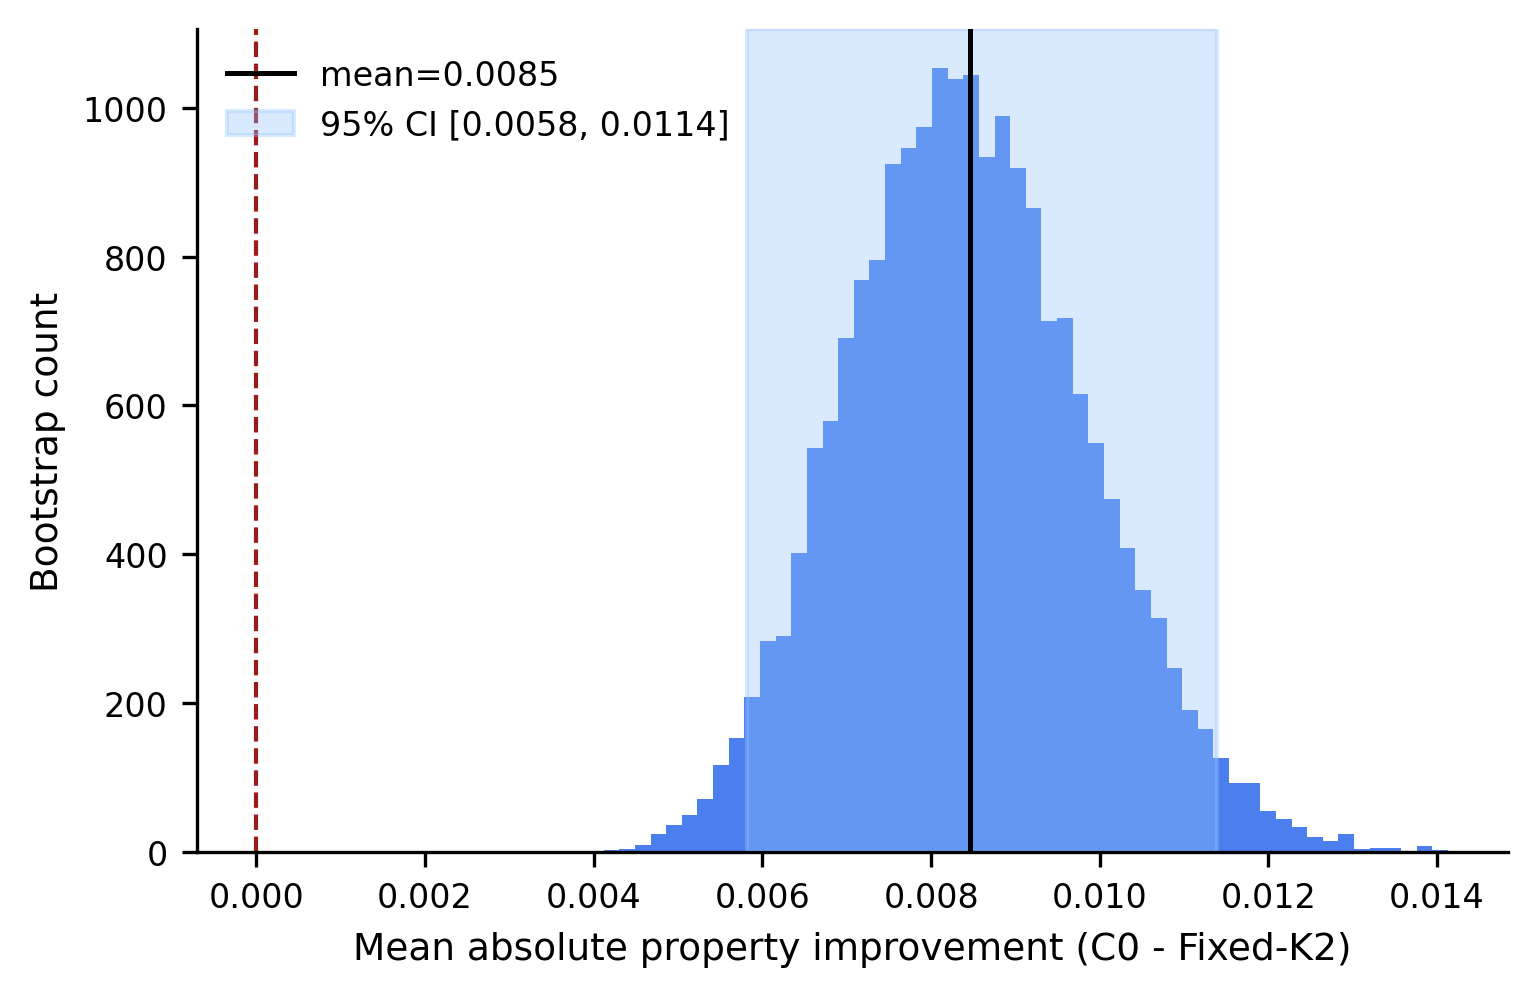
\includegraphics[keepaspectratio,alt={图3-4 Fixed-K2 相对 C0 的 20 000 次配对自助法增益分布}]{../../../thesis_release/innovation1/figures/I1_F3_fixed_gain_bootstrap.png}}
\bicaption{Fixed-K2 相对 C0 的 20 000 次配对自助法增益分布}{20,000 Paired-Bootstrap Gain Distribution of Fixed-K2 Relative to C0}
\end{figure}

\subsection{质量护栏与计算代价}

Fixed-K2 的平均 E-hull 从 0.104296 降至 0.081135 eV/atom，Stable 从 58.59\% 增至 70.31\%，NUS 从 32.81\% 增至 37.50\%，Validity 保持 100\%，没有违反冻结的代理质量护栏。图3-5给出主要质量指标对比。

\begin{figure}
\centering
\pandocbounded{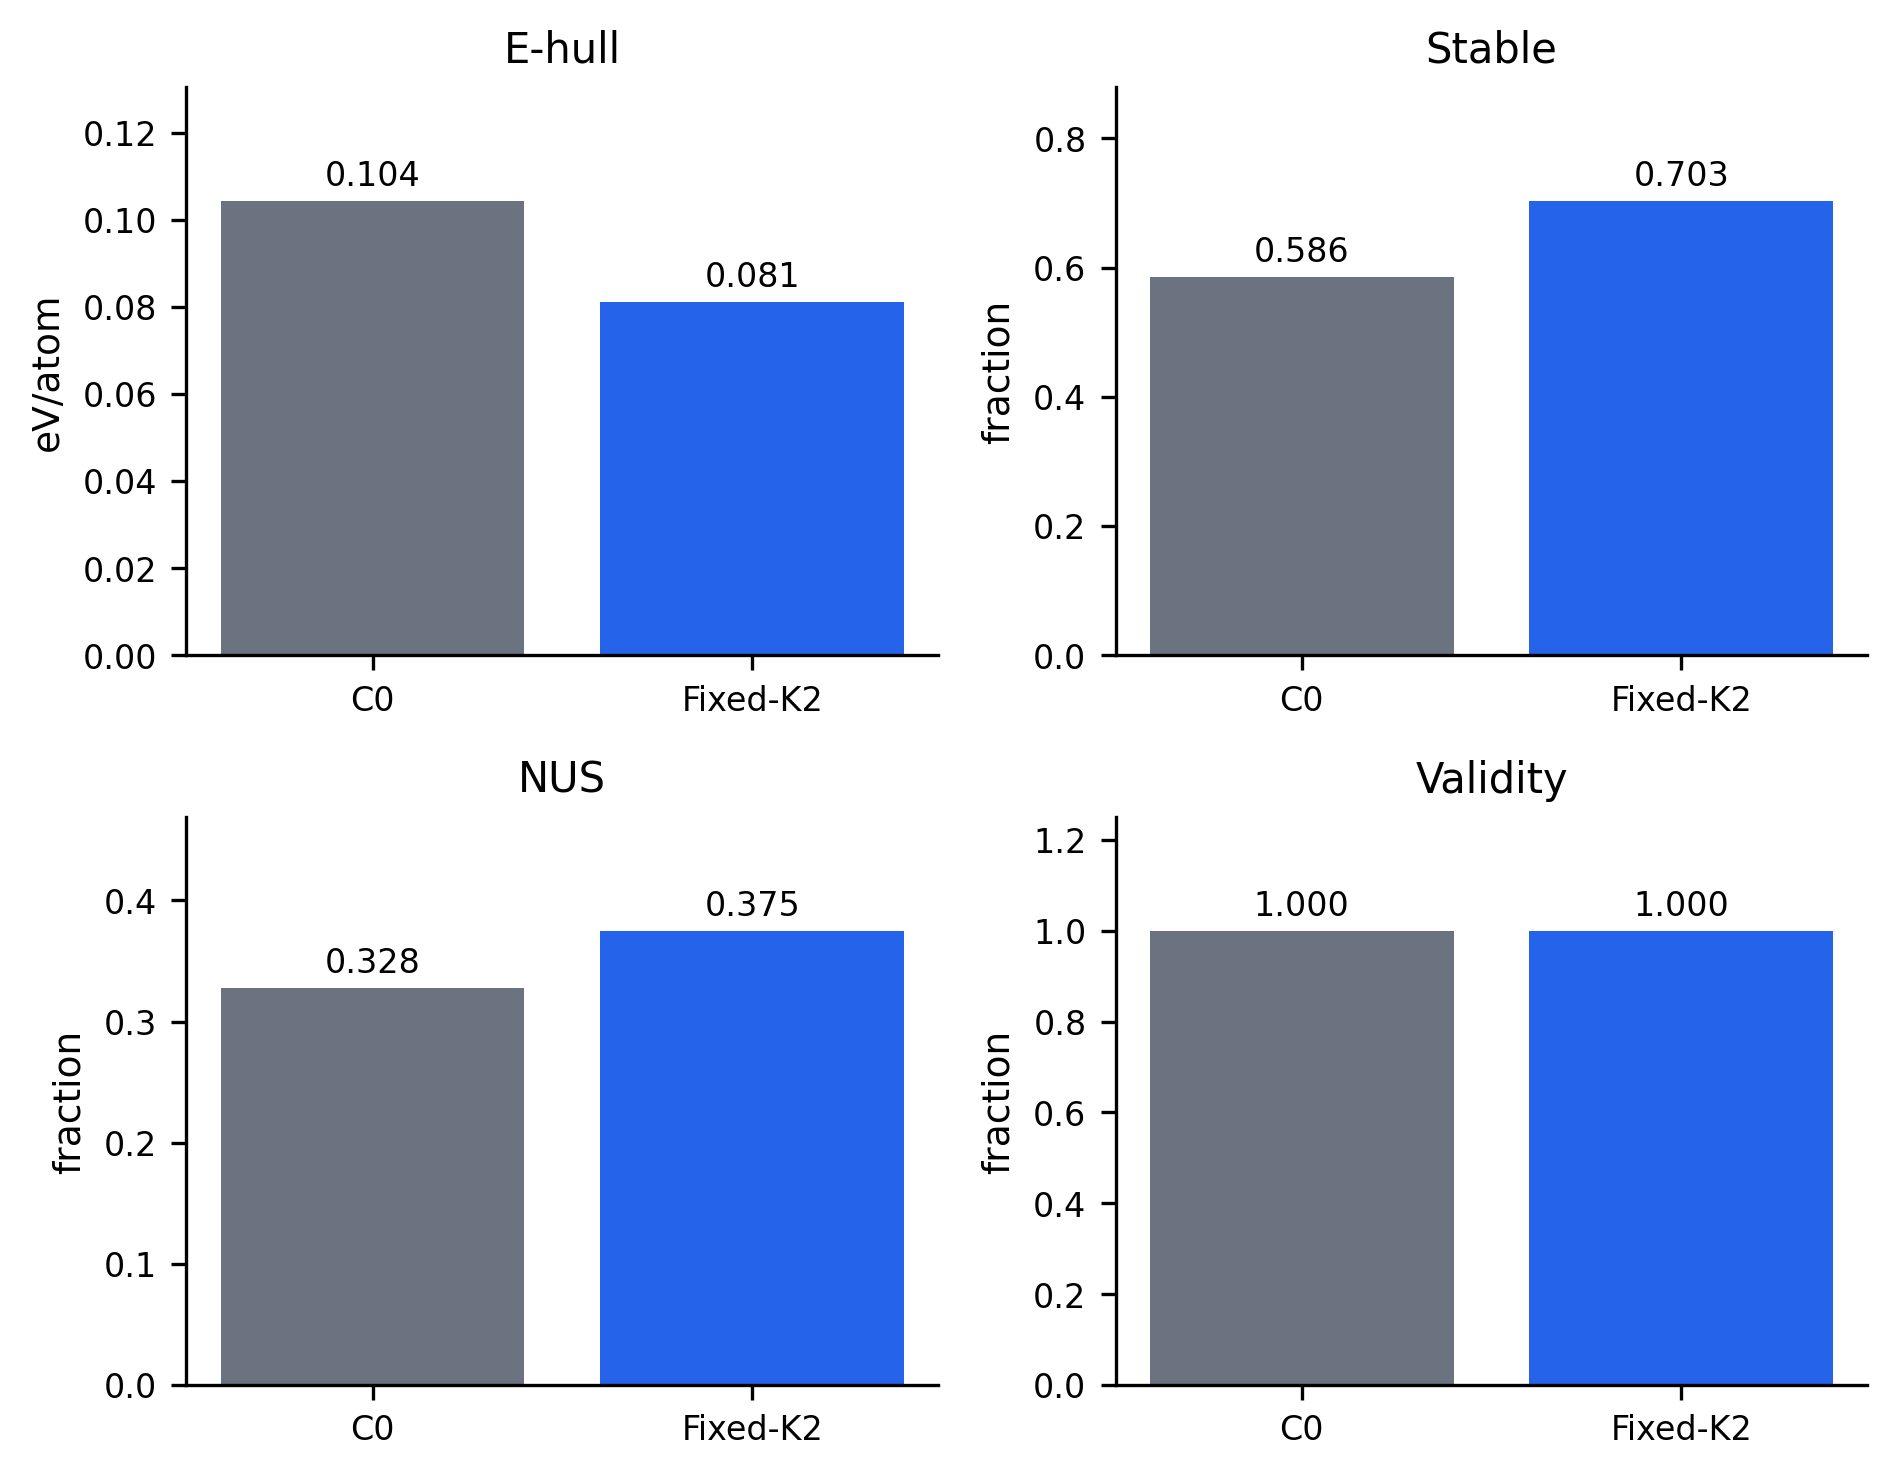
\includegraphics[keepaspectratio,alt={图3-5 C1-128 的代理质量护栏结果}]{../../../thesis_release/innovation1/figures/I1_F4_quality_guardrails.png}}
\bicaption{C1-128 的代理质量护栏结果}{Proxy Quality Guardrails on C1-128}
\end{figure}

上述``0 个属性损失''应结合算法定义解释：Fixed-K2 只有在终点属性严格改善且质量条件通过时才接受候选，否则返回精确 C0。因此，它证明的是终点约束选择和参考回退在该代理协议下按设计工作，而不是证明每个候选分支本身从不失败。事实上，回退率为 58.59\%，说明大部分样本仍保留 C0。

计算代价方面，Fixed-K2 每个样本需要 4 400 次 MatterGen 得分调用和 3 次终点评价，对应约 2.2 倍 C0 计算量。图3-6区分了部署成本与 Phase B 数据构建成本。该结果不能表述为 Fixed-K2 在相同的 1.0 倍预算下优于 C0，而应表述为在固定 2.2 倍推理预算下，以额外计算换取终点验证和保守回退。

\begin{figure}
\centering
\pandocbounded{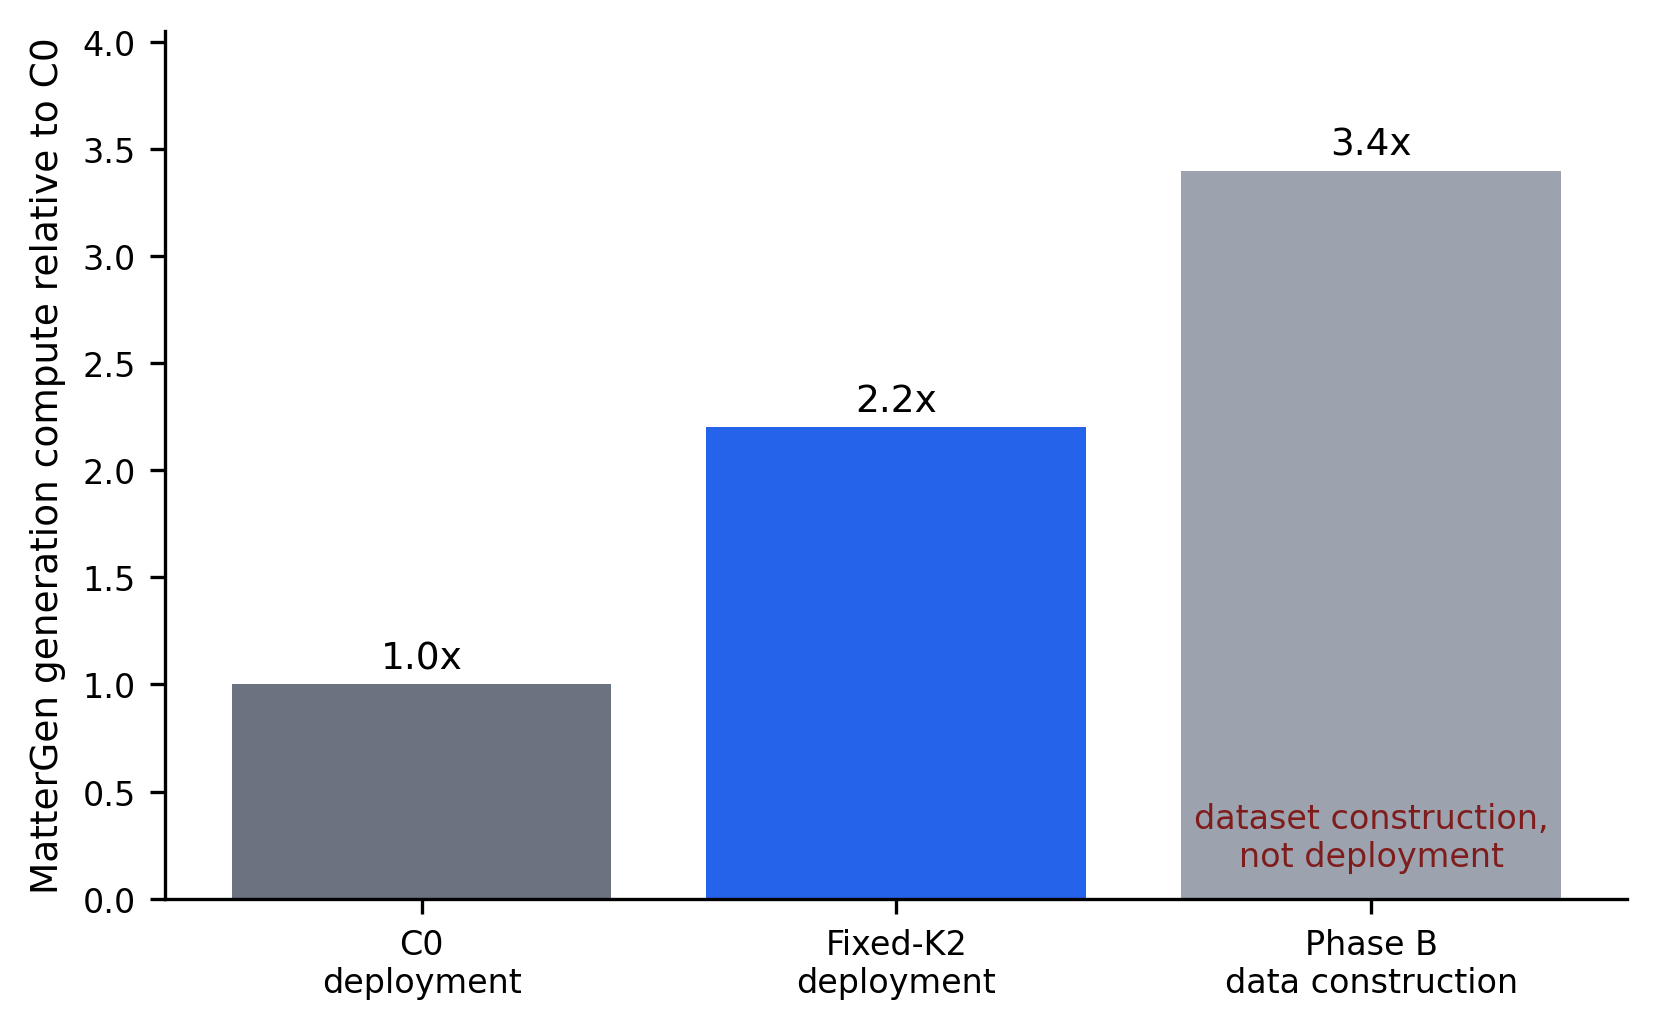
\includegraphics[keepaspectratio,alt={图3-6 C0、Fixed-K2 及 Phase B 数据构建的计算量比较}]{../../../thesis_release/innovation1/figures/I1_F5_compute_comparison.png}}
\bicaption{C0、Fixed-K2 及 Phase B 数据构建的计算量比较}{Computational Cost Comparison of C0, Fixed-K2, and Phase B Data Construction}
\end{figure}

\section{学习型 Linear-K2 分配器的负消融}

\subsection{Phase B 候选分配实验}

Fixed-K2 对所有样本分配相同的 GPulse 与 PPulse。为检验分支点特征能否支持样本级候选分配，Phase B 使用 64 个全新种子构建数据集，并按 32/16/16 划分训练集、验证集和测试集。每个样本在第 400 步提取 179 个无终点信息泄漏的分支前特征，包括三个字段在预测器/校正器阶段的残差、条件与无条件得分范数、对齐度、25/50/100 步窗口统计以及分支状态的结构描述量。加入策略交互后形成 895 个数值设计列，再加策略独热编码共 899 个设计列。

验证集最终选择 \(C=1.0\)、类别平衡的线性逻辑分配器 Linear-K2。它为四个候选估计``安全且有益''的概率，并生成概率最高的两个后缀。Phase B 的 16 个留出测试样本上，Linear-K2 的 Property MAE 为 0.023634，Fixed-K2 为 0.024597，方向性相对改善 3.92\%；但两者配对增益的 20 000 次自助法 95\% 区间为 \([-0.002618,0.005214]\)，跨越零，未达到预注册的分配器优势门槛。因此 Phase B 的冻结结论为 \texttt{ADAPTIVE\_ALLOCATION\_VALUE=NOT\_SUP\allowbreak PORTED}，不能将该小样本方向性结果写为已验证的学习型优势。

\subsection{模型重建与冻结}

Phase B 当时未保存 scikit-learn 序列化模型。为进行独立确认，在注册任何新确认种子之前，使用原始训练集 32 个样本、原始冻结代码、原始 179 个特征和已确定的 \(C=1.0\) 进行了一次确定性重建。重建模型对 16 个历史测试种子的 Top-2 候选选择实现 16/16 完全一致，验证/测试指标的最大绝对误差为 \(1.11\times10^{-16}\)。通过后，模型被标记为 \texttt{RECONSTRUCTED\_ARTIFACT} 并以 SHA-256 \texttt{bd3f5280\allowbreak957a6418\allowbreak e7d5275a\allowbreak3e7a576f\allowbreak c57872b3\allowbreak ad1bd19ae\allowbreak e9ef7bef\allowbreak97d56d3a} 永久冻结。该过程只恢复缺失的序列化对象，不改变模型、特征、超参数或 Phase B 的历史负结论。

\subsection{C1-128 独立确认}

在 C1 的 128 个完全新种子上，Linear-K2 的 Property MAE 为 0.027522，反而高于 Fixed-K2 的 0.026332。以 \(E_{\mathrm{Fixed}}-E_{\mathrm{Linear}}\) 定义 Linear-K2 的配对增益，其均值为 \(-0.001190\)，相对增益为 \(-4.52\%\)，20 000 次自助法 95\% 区间为 \([-0.003148,0.000740]\)。逐样本胜/平/负为 31/62/35。虽然 Linear-K2 相对 C0 仍因终点约束与回退获得较低误差，但本实验的主要问题是它能否在相同 2.2 倍预算下优于 Fixed-K2；对此，方向和置信区间均不支持肯定结论。

C1 的继续门槛要求 Linear-K2 严格优于 Fixed-K2、相对改善至少 1\%、不劣于 Random-\allowbreak K2，并通过质量护栏。前两项失败，故冻结结论为 \texttt{FROZEN\_LINEAR\_K2\_CONFIRMATION=NOT\_SUP\allowbreak PORTED}，C2 按协议不运行，也未进行结果后的补救调参。该负结果说明，在当前特征表示、训练规模和候选库下，学习型样本分配没有独立确认优于 Fixed-K2。

\section{讨论}

\subsection{科学结论}

第一，引导优化空间客观存在。V3 的完整终点 Oracle 在不同样本与时刻同时选择降低、保持和提高 CFG，并取得 27.22\% 的回顾性改善；分支兼容 Oracle 在合法共享前缀条件下仍显示 30.41\% 的测试集改善。这些结果排除了``固定 CFG=2.0 对所有样本均已最优''的解释。

第二，在线识别是比优化空间本身更困难的问题。V1 的残差反馈缺乏跨批次稳定性；经过时间归一化、中位数聚合、置信回退和限速的 V2 仍未降低伤害率；V4/V5 的风险与安全模型不能同时满足覆盖率和伤害门槛；V3 的短视野标签也不能预测完整终点结果。这些相互独立的证据指向同一问题：中间状态中易于构造的局部统计量，与最终属性---质量结果之间存在不足以支持可靠控制的代理错配。

第三，在当前证据下，简单固定预算分支比学习型分配更稳健。Fixed-K2 不需要由分支前特征决定候选身份，而是始终展开 GPulse 与 PPulse，再利用终点评价作出选择。它在全新 C1-128 上得到正的配对改善区间，并通过冻结质量护栏；Linear-K2 则未在相同预算下确认优于 Fixed-K2。这并不否定未来使用更强状态表征或更多训练数据的可能性，但说明当前没有必要以更复杂的学习型分配器替代固定策略。

第四，参考轨迹保留将不确定控制转化为保守选择。只要 C0 被精确保留，候选失败就不必被写入最终输出；终点选择能够利用完整结果，而不依赖短视野代理。该设计的实质贡献不在于宣称找到了普适最优 CFG，而在于改变风险承担方式：从单轨迹上的不可逆在线动作，转化为有限候选中的终点约束决策。

\subsection{局限性}

本章方法仍存在以下边界。

\begin{enumerate}
\def\labelenumi{\arabic{enumi}.}
\tightlist
\item
  Fixed-K2 的 MatterGen 得分调用约为 C0 的 2.2 倍，并额外需要候选终点评价。它以计算换取选择可靠性，不是推理加速方法。
\item
  方法依赖终点属性与质量评价器。若代理模型存在系统偏差，接受规则也可能继承该偏差。
\item
  Fixed-K2 不是纯在线、单轨迹的 Adaptive CFG。它需要保存状态、复制后缀并在生成完成后选择。
\item
  学习型样本级候选分配未得到支持。Linear-K2 的 Phase B 方向性结果没有通过门槛，C1 独立确认也未优于 Fixed-K2。
\item
  当前属性、E-hull、稳定性及相关质量判断主要依赖 CHGNet 与 Matter\allowbreak Sim 代理模型，没有进行 DFT 或实验验证，不能据此证明材料的真实物理稳定性或可合成性。
\item
  本研究没有设置所有可能的等预算通用多样本筛选基线，因此没有证明 Fixed-K2 优于每一种 2.2 倍预算的通用 best-of-N 方法。
\item
  候选库、分支点和终点阈值均在当前 MatterGen 条件任务上冻结，跨属性、跨材料域和跨生成模型的迁移性仍需独立研究。
\end{enumerate}

上述边界也限定了本章的创新表述：本文提出并验证的是面向当前 MatterGen 条件任务的参考轨迹保留、固定预算、终点约束选择框架，而不主张首次提出多分支扩散或验证器引导晶体生成，也不作普适最优或物理安全保证。

\section{本章小结}

本章从固定 CFG 的局限出发，首先提出多字段残差驱动的在线自适应引导。历史 Formal256 呈现方向性质量改善，但新样本没有稳定复现，说明直接残差控制存在跨批次稳定性问题。反事实 Oracle 随后证明，更优的样本级与时刻级引导客观存在；然而，短视野标签、稳健残差变换、风险校准、安全选择、阶段门控和字段解耦均未形成可靠的在线识别策略。

基于这些证据，本文将研究问题由``提前预测最优引导''转化为``在有限预算内保留参考轨迹并验证少量候选''，形成参考轨迹保留的预算约束多分支条件引导与安全回退方法。该方法在第 400 步保存完整采样与 RNG 状态，保留精确 C0，并以固定预算展开 GPulse 和 PPulse 两个候选；只有候选同时实现属性改进并满足预定义质量约束时才被接受，否则执行参考回退并返回 C0。

在 128 个完全独立确认样本上，Fixed-K2 将 Property MAE 从 0.034796 降至 0.026332，相对改善 24.32\%，20 000 次配对自助法的绝对改善区间为 \([0.005817,0.011391]\)，同时满足冻结的代理质量护栏。进一步的 Linear-K2 实验未能在相同预算下独立确认优于 Fixed-K2，因此最终选择固定双候选分支策略作为本章方法。完整证据支持``有限预算的参考保留与终点选择有效''，但不支持``在线 Adaptive CFG 已被稳定验证''或``学习型候选分配具有额外价值''。本章主要解决条件属性控制问题；属性条件满足并不等价于生成结构处于低受力状态，因此第4章进一步研究后期神经力场反馈对局部结构一致性的影响。
